% Created by tikzDevice version 0.12.6 on 2024-07-27 08:35:26
% !TEX encoding = UTF-8 Unicode
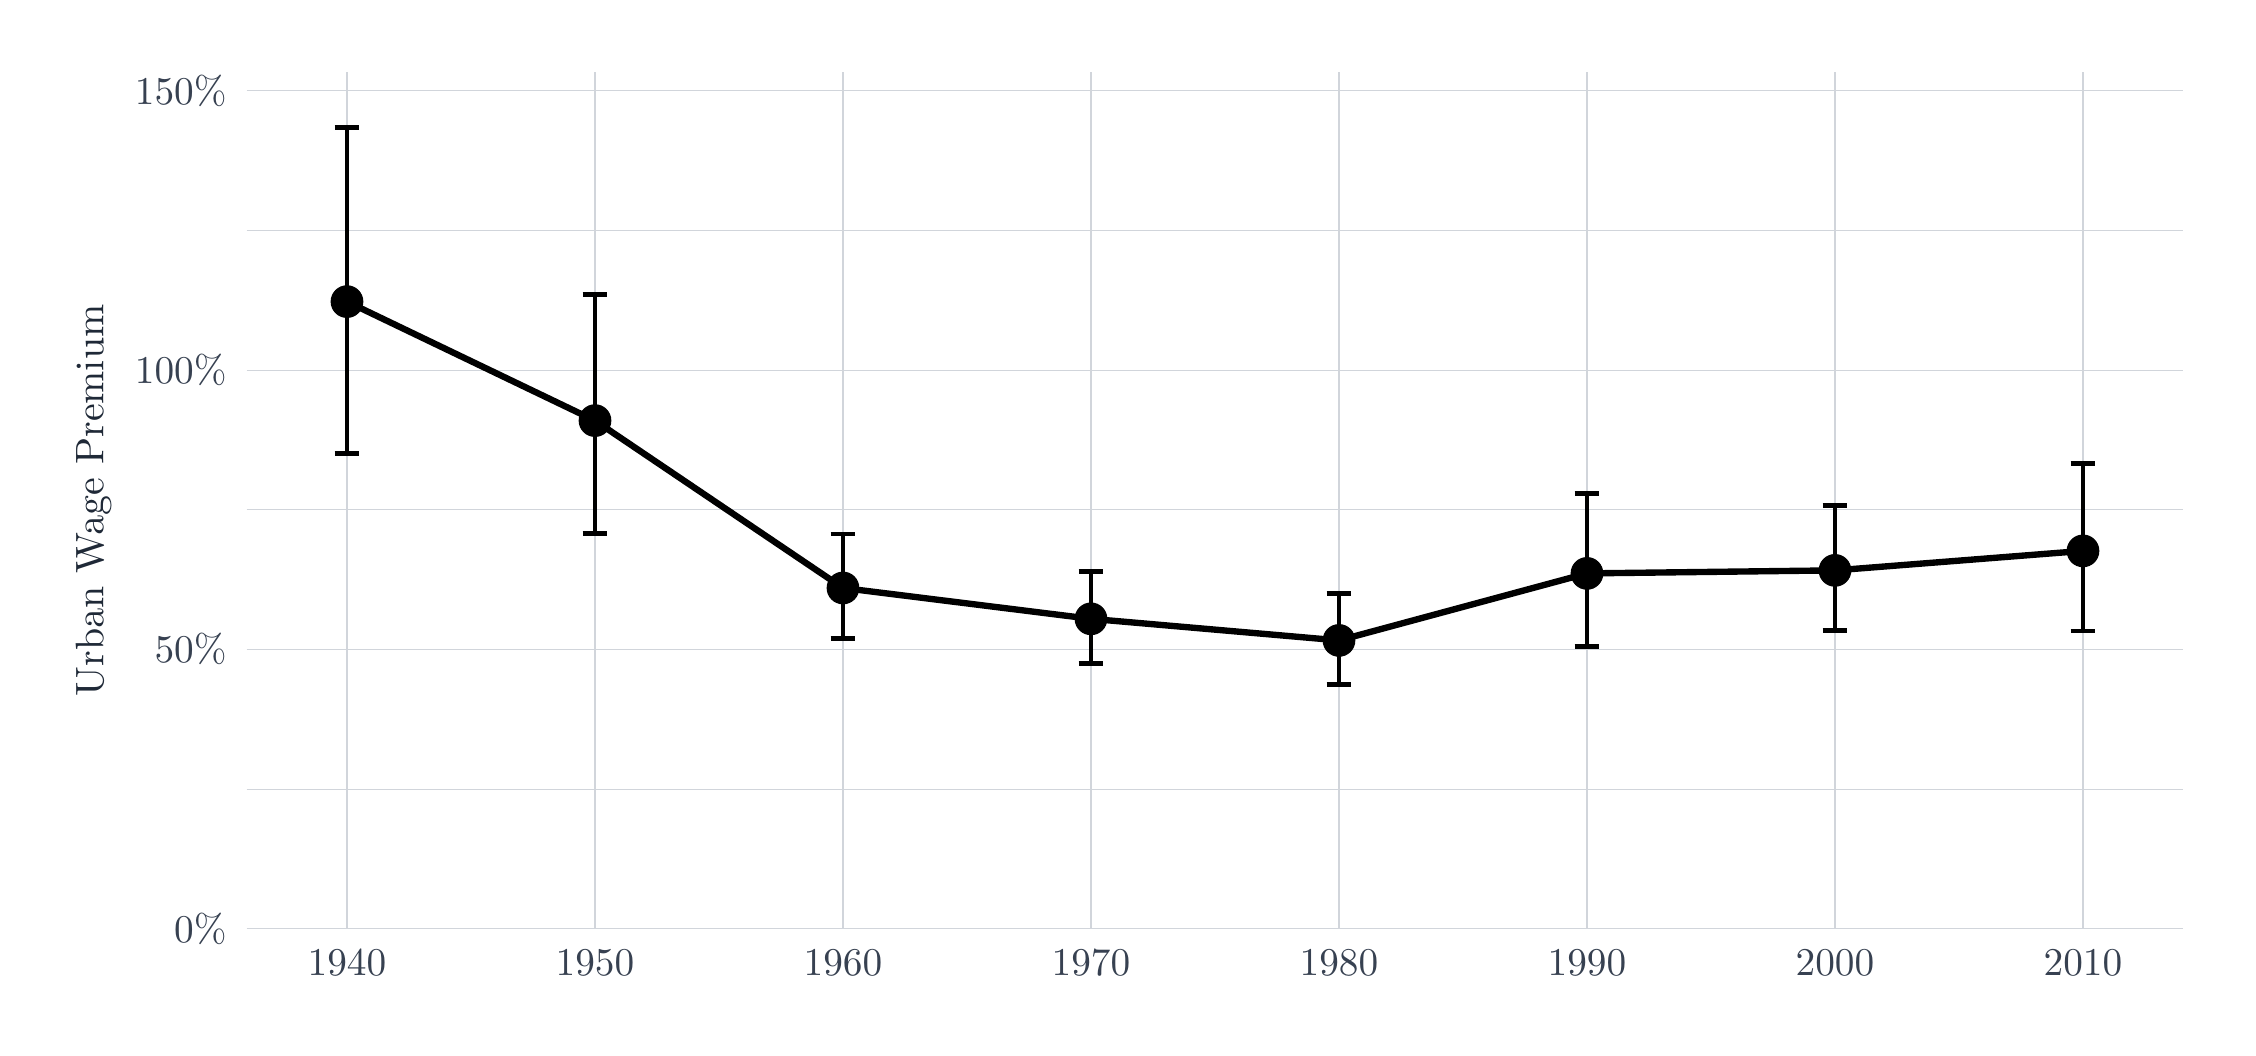
\begin{tikzpicture}[x=1pt,y=1pt]
\definecolor{fillColor}{RGB}{255,255,255}
\path[use as bounding box,fill=fillColor] (0,0) rectangle (794.97,361.35);
\begin{scope}
\path[clip] (  0.00,  0.00) rectangle (794.97,361.35);
\definecolor{drawColor}{RGB}{255,255,255}

\path[draw=drawColor,line width= 0.8pt,line join=round,line cap=round,fill=fillColor] (  0.00,  0.00) rectangle (794.97,361.35);
\end{scope}
\begin{scope}
\path[clip] ( 79.09, 35.76) rectangle (778.97,345.35);
\definecolor{drawColor}{RGB}{255,255,255}
\definecolor{fillColor}{RGB}{255,255,255}

\path[draw=drawColor,line width= 0.8pt,line join=round,line cap=round,fill=fillColor] ( 79.09, 35.76) rectangle (778.97,345.35);
\definecolor{drawColor}{RGB}{209,213,219}

\path[draw=drawColor,line width= 0.4pt,line join=round] ( 79.09, 86.22) --
	(778.97, 86.22);

\path[draw=drawColor,line width= 0.4pt,line join=round] ( 79.09,187.14) --
	(778.97,187.14);

\path[draw=drawColor,line width= 0.4pt,line join=round] ( 79.09,288.06) --
	(778.97,288.06);

\path[draw=drawColor,line width= 0.4pt,line join=round] ( 79.09, 35.76) --
	(778.97, 35.76);

\path[draw=drawColor,line width= 0.4pt,line join=round] ( 79.09,136.68) --
	(778.97,136.68);

\path[draw=drawColor,line width= 0.4pt,line join=round] ( 79.09,237.60) --
	(778.97,237.60);

\path[draw=drawColor,line width= 0.4pt,line join=round] ( 79.09,338.52) --
	(778.97,338.52);

\path[draw=drawColor,line width= 0.4pt,line join=round] (115.38, 35.76) --
	(115.38,345.35);

\path[draw=drawColor,line width= 0.4pt,line join=round] (205.00, 35.76) --
	(205.00,345.35);

\path[draw=drawColor,line width= 0.4pt,line join=round] (294.61, 35.76) --
	(294.61,345.35);

\path[draw=drawColor,line width= 0.4pt,line join=round] (384.22, 35.76) --
	(384.22,345.35);

\path[draw=drawColor,line width= 0.4pt,line join=round] (473.84, 35.76) --
	(473.84,345.35);

\path[draw=drawColor,line width= 0.4pt,line join=round] (563.45, 35.76) --
	(563.45,345.35);

\path[draw=drawColor,line width= 0.4pt,line join=round] (653.06, 35.76) --
	(653.06,345.35);

\path[draw=drawColor,line width= 0.4pt,line join=round] (742.68, 35.76) --
	(742.68,345.35);
\definecolor{drawColor}{RGB}{0,0,0}

\path[draw=drawColor,line width= 2.3pt,line join=round] (115.38,262.36) --
	(205.00,219.36) --
	(294.61,158.88) --
	(384.22,147.73) --
	(473.84,139.93) --
	(563.45,164.15) --
	(653.06,165.24) --
	(742.68,172.28);

\path[draw=drawColor,line width= 1.7pt,line join=round] (110.90,325.17) --
	(119.86,325.17);

\path[draw=drawColor,line width= 1.7pt,line join=round] (115.38,325.17) --
	(115.38,207.59);

\path[draw=drawColor,line width= 1.7pt,line join=round] (110.90,207.59) --
	(119.86,207.59);

\path[draw=drawColor,line width= 1.7pt,line join=round] (200.52,265.04) --
	(209.48,265.04);

\path[draw=drawColor,line width= 1.7pt,line join=round] (205.00,265.04) --
	(205.00,178.52);

\path[draw=drawColor,line width= 1.7pt,line join=round] (200.52,178.52) --
	(209.48,178.52);

\path[draw=drawColor,line width= 1.7pt,line join=round] (290.13,178.34) --
	(299.09,178.34);

\path[draw=drawColor,line width= 1.7pt,line join=round] (294.61,178.34) --
	(294.61,140.52);

\path[draw=drawColor,line width= 1.7pt,line join=round] (290.13,140.52) --
	(299.09,140.52);

\path[draw=drawColor,line width= 1.7pt,line join=round] (379.74,164.71) --
	(388.70,164.71);

\path[draw=drawColor,line width= 1.7pt,line join=round] (384.22,164.71) --
	(384.22,131.62);

\path[draw=drawColor,line width= 1.7pt,line join=round] (379.74,131.62) --
	(388.70,131.62);

\path[draw=drawColor,line width= 1.7pt,line join=round] (469.36,156.79) --
	(478.32,156.79);

\path[draw=drawColor,line width= 1.7pt,line join=round] (473.84,156.79) --
	(473.84,123.95);

\path[draw=drawColor,line width= 1.7pt,line join=round] (469.36,123.95) --
	(478.32,123.95);

\path[draw=drawColor,line width= 1.7pt,line join=round] (558.97,193.01) --
	(567.93,193.01);

\path[draw=drawColor,line width= 1.7pt,line join=round] (563.45,193.01) --
	(563.45,137.61);

\path[draw=drawColor,line width= 1.7pt,line join=round] (558.97,137.61) --
	(567.93,137.61);

\path[draw=drawColor,line width= 1.7pt,line join=round] (648.58,188.63) --
	(657.54,188.63);

\path[draw=drawColor,line width= 1.7pt,line join=round] (653.06,188.63) --
	(653.06,143.39);

\path[draw=drawColor,line width= 1.7pt,line join=round] (648.58,143.39) --
	(657.54,143.39);

\path[draw=drawColor,line width= 1.7pt,line join=round] (738.20,203.87) --
	(747.16,203.87);

\path[draw=drawColor,line width= 1.7pt,line join=round] (742.68,203.87) --
	(742.68,143.38);

\path[draw=drawColor,line width= 1.7pt,line join=round] (738.20,143.38) --
	(747.16,143.38);
\definecolor{fillColor}{RGB}{0,0,0}

\path[draw=drawColor,line width= 0.4pt,line join=round,line cap=round,fill=fillColor] (115.38,262.36) circle (  5.71);

\path[draw=drawColor,line width= 0.4pt,line join=round,line cap=round,fill=fillColor] (205.00,219.36) circle (  5.71);

\path[draw=drawColor,line width= 0.4pt,line join=round,line cap=round,fill=fillColor] (294.61,158.88) circle (  5.71);

\path[draw=drawColor,line width= 0.4pt,line join=round,line cap=round,fill=fillColor] (384.22,147.73) circle (  5.71);

\path[draw=drawColor,line width= 0.4pt,line join=round,line cap=round,fill=fillColor] (473.84,139.93) circle (  5.71);

\path[draw=drawColor,line width= 0.4pt,line join=round,line cap=round,fill=fillColor] (563.45,164.15) circle (  5.71);

\path[draw=drawColor,line width= 0.4pt,line join=round,line cap=round,fill=fillColor] (653.06,165.24) circle (  5.71);

\path[draw=drawColor,line width= 0.4pt,line join=round,line cap=round,fill=fillColor] (742.68,172.28) circle (  5.71);
\end{scope}
\begin{scope}
\path[clip] (  0.00,  0.00) rectangle (794.97,361.35);
\definecolor{drawColor}{RGB}{55,65,81}

\node[text=drawColor,anchor=base east,inner sep=0pt, outer sep=0pt, scale=  1.42] at ( 71.89, 30.86) {0\%};

\node[text=drawColor,anchor=base east,inner sep=0pt, outer sep=0pt, scale=  1.42] at ( 71.89,131.78) {50\%};

\node[text=drawColor,anchor=base east,inner sep=0pt, outer sep=0pt, scale=  1.42] at ( 71.89,232.70) {100\%};

\node[text=drawColor,anchor=base east,inner sep=0pt, outer sep=0pt, scale=  1.42] at ( 71.89,333.62) {150\%};
\end{scope}
\begin{scope}
\path[clip] (  0.00,  0.00) rectangle (794.97,361.35);
\definecolor{drawColor}{RGB}{55,65,81}

\node[text=drawColor,anchor=base,inner sep=0pt, outer sep=0pt, scale=  1.42] at (115.38, 18.76) {1940};

\node[text=drawColor,anchor=base,inner sep=0pt, outer sep=0pt, scale=  1.42] at (205.00, 18.76) {1950};

\node[text=drawColor,anchor=base,inner sep=0pt, outer sep=0pt, scale=  1.42] at (294.61, 18.76) {1960};

\node[text=drawColor,anchor=base,inner sep=0pt, outer sep=0pt, scale=  1.42] at (384.22, 18.76) {1970};

\node[text=drawColor,anchor=base,inner sep=0pt, outer sep=0pt, scale=  1.42] at (473.84, 18.76) {1980};

\node[text=drawColor,anchor=base,inner sep=0pt, outer sep=0pt, scale=  1.42] at (563.45, 18.76) {1990};

\node[text=drawColor,anchor=base,inner sep=0pt, outer sep=0pt, scale=  1.42] at (653.06, 18.76) {2000};

\node[text=drawColor,anchor=base,inner sep=0pt, outer sep=0pt, scale=  1.42] at (742.68, 18.76) {2010};
\end{scope}
\begin{scope}
\path[clip] (  0.00,  0.00) rectangle (794.97,361.35);
\definecolor{drawColor}{RGB}{31,41,55}

\node[text=drawColor,rotate= 90.00,anchor=base,inner sep=0pt, outer sep=0pt, scale=  1.44] at ( 27.32,190.55) {Urban Wage Premium};
\end{scope}
\end{tikzpicture}
